\section{Tools}
\label{section:bcoollengbench}
\bcool is developed as set of plugins for Eclipse Modeling Framework (EMF)\footnote{http://www.eclipse.org}. Its abstract syntax has been developed using Ecore (\ie the meta-language associated with EMF) and the textual concrete  syntax has been developed in Xtext, thus providing advanced editing facilities (see Figure~\ref{fig:bcooltechnos}). A \bcool specification is defined between languages by relying on its language behavioral interface made of \dse. To get the \dse, the \ecl specification of each language must be imported (Figure~\ref{fig:bcooltechnos}: point 1). From a \bcool specification, the generation of the coordination between models has been automated by relying on two technologies: Acceleo\footnote{http://www.eclipse.org/acceleo/} and QVTo\footnote{https://projects.eclipse.org/projects/modeling.mmt.qvt-oml}. The acceleo transformation translates the \bcool specification into a QVTo transformation (Figure~\ref{fig:bcooltechnos}: point 2). The transformation can be applied between models to generate the coordination specification in \ccsl (Figure~\ref{fig:bcooltechnos}: point 3).    
	
\begin{figure}[h]
		\begin{center}
			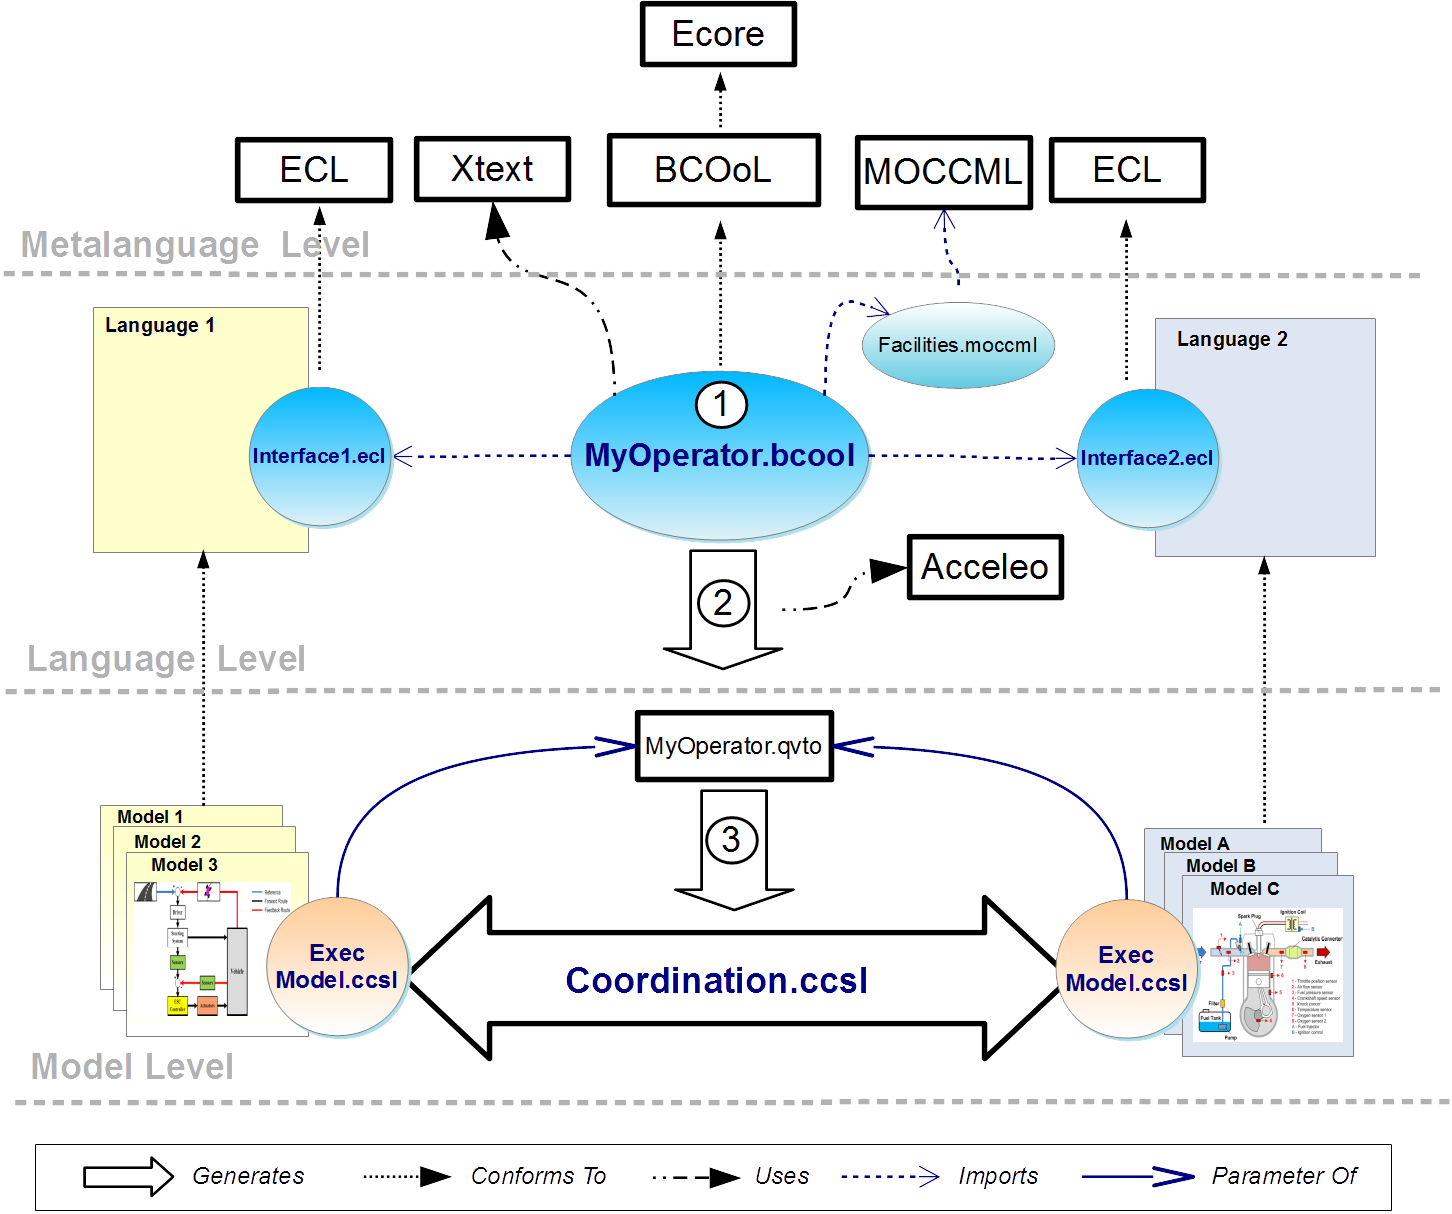
\includegraphics[width=1\textwidth]{bcool/figs/bcooltechnos.png}
			\caption{\bcool Tooling Technologies}
			\label{fig:bcooltechnos}
		\end{center}
\end{figure}
	
These technologies has been integrated into the GEMOC Studio, an Eclipse package atop EMF, which includes both a \emph{language workbench} to design and implement tool-supported xDSMLs, and a \emph{modeling workbench} where the xDSMLs are automatically deployed to allow system designers to edit, execute, simulate, and animate their models. In this context, \bcool takes advantages of this collaborative environment by adding coordination facilities. 

\begin{figure}[h]
	\begin{center}
		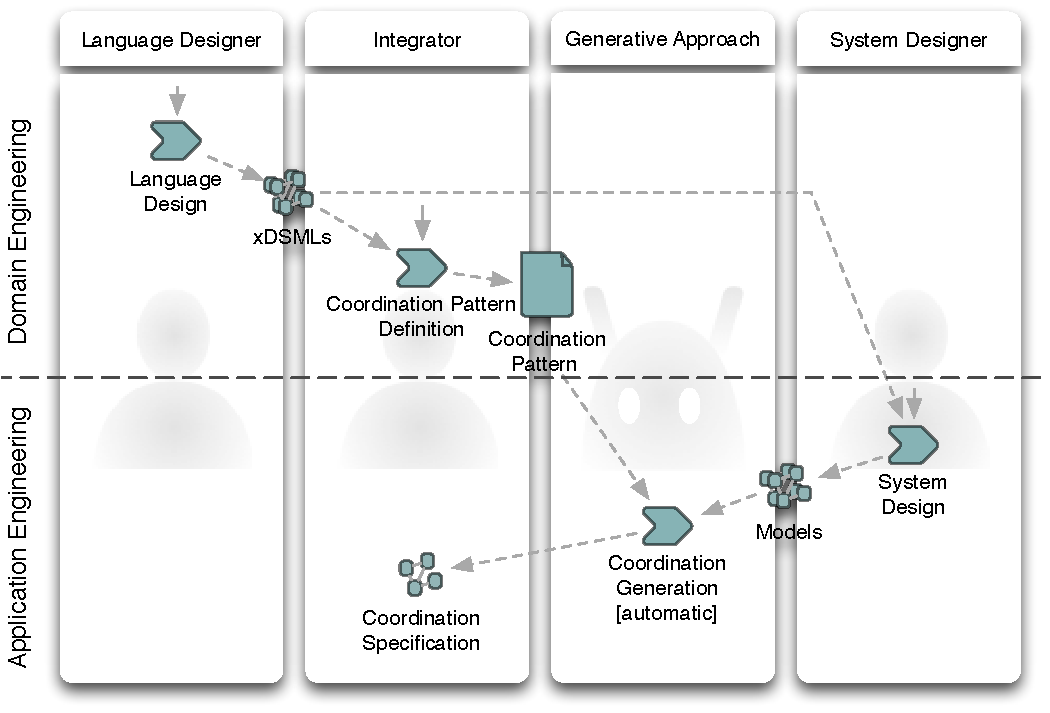
\includegraphics[width=.6\textwidth]{bcool/figs/process}
		\caption{The Proposed Workflow}
		\label{fig:proposedworkflow}
	\end{center}
\end{figure}

Based on the GEMOC studio, Figure~\ref{fig:proposedworkflow} illustrates the proposed workflow. Such a workflow relies mainly in two stakeholders: an integrator that uses the language workbench and an system designer that uses the model workbench. 

In the language workbench, an integrator develop operators by relying on the deployed languages. The \bcool specification can import the language behavioral interface that are automatically deployed into the workbench. To build its own libraries, the workbench provides \moccml thus helping the integrator to specify EventRelations and EventExpression. 

Operators are automatically deployed into the modeling workbench and can be used by a system designer to generate the coordination. This task is automated by relying on a set of plugins\footnote{\todo{I have to talk about how the operators are applied by the plugin, this is not evident!}}. The workbench provides several tools to perform verification activities \eg execution and animation, space-state exploration, etc.  

To summarize, a \bcool developer (\ie integrator) develops a set of operators by relying on the language behavioral interface (\ecl) and libraries (\moccml). Then, a \bcool user (\ie system designer) applies these operator on his models to: 
		\begin{itemize}
			\item Generate a coordination specification.
			\item Perform execution and verification activities.
		\end{itemize}

We implement the running example in the GEMOC studio. We rely on the languages TFSM and Activity that are integrated into the study. Then, we use \bcool to specify the operator in Listing~\ref{lst:bcoolrunningexample} (Figure~\ref{fig:screenbcool}: point 1). In the model workbench, we build the models of the coffee machine: a TFSM named \emph{CoffeeCoin} and an Activity named \emph{CoffeeAlgorithm} (Figure~\ref{fig:screenbcool}: point 2). Then, we use the workbench to execute, verify and animate the coordinated models. In particular, Figure shows the animation proposed by Sirius.   

\begin{figure}[h]
	\begin{center}
		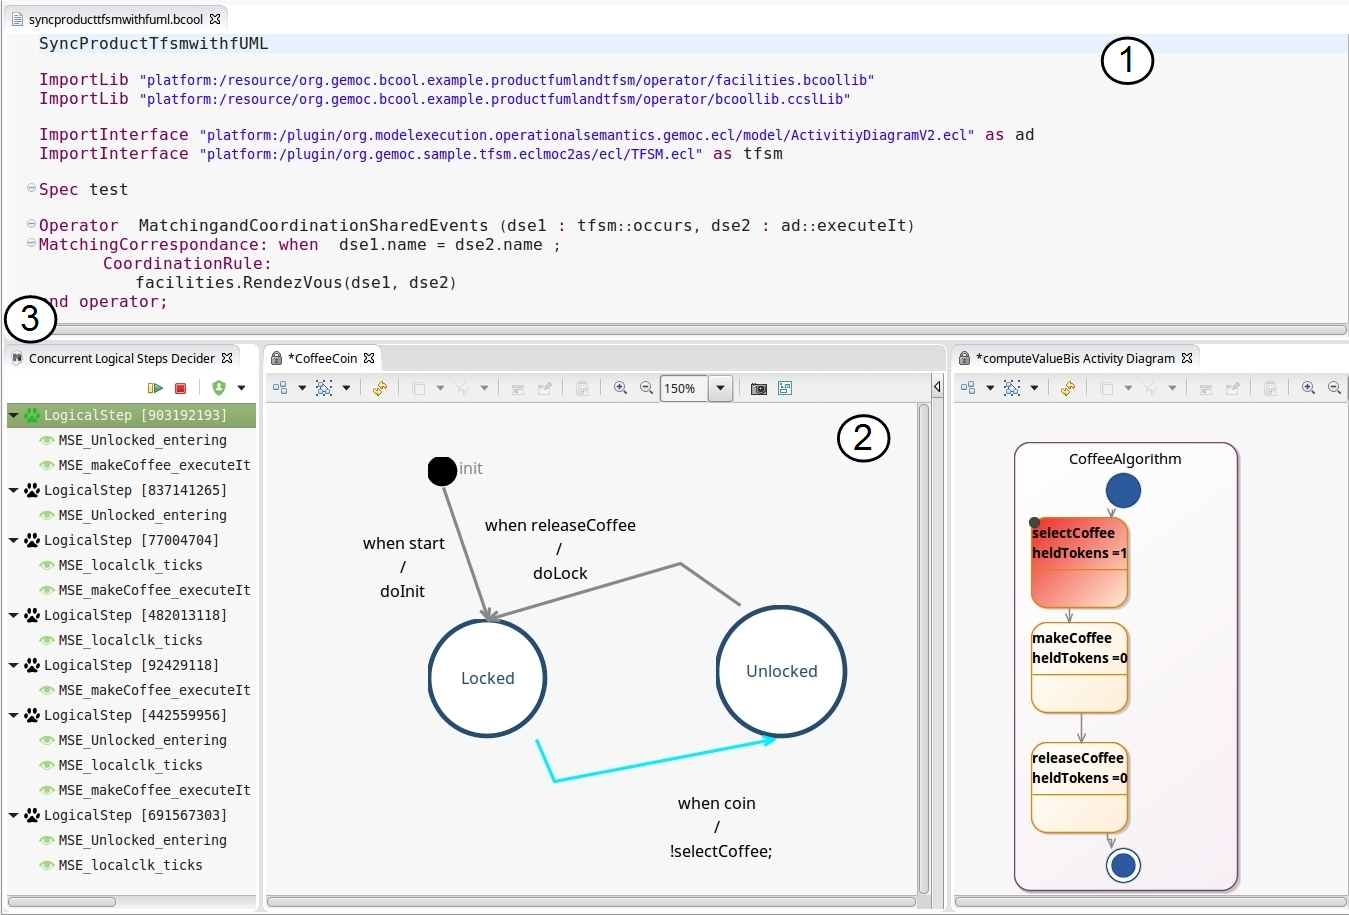
\includegraphics[width=.6\textwidth]{bcool/figs/bcoolscreen.png}
		\caption{Screenshot}
		\label{fig:screenbcool}
	\end{center}
\end{figure}

A video presenting the whole flow can be found on the companion website~\footnote{http://timesquare.inria.fr/BCOoL}, which also contains more examples with full descriptions. These examples are hosted in Github~\footnote{http://github.com} at BCOoLExamples~\footnote{http://matiasvara.github.io/BCOoLExamples/}. The \bcool code is hosted in the open source project Gemoc~\footnote{http://github.com/gemoc/} thus making the project fully available.

  

